\documentclass[12pt]{article}

\usepackage{autres/imports}
\usepackage{autres/pseudocode}
\usepackage{autres/renews}

\begin{document}

%page de garde
 \begin{titlepage}


    \centering{

    \textbf{Algorithmique Avancée et Programmation C}
  
    \noindent\rule{16.5cm}{0.5pt}

    \vspace{50px}
    
    \Huge
    Projet Compresseur d'Huffman
    
    \normalsize
    
    \vspace{270px}
    \textbf{Réalisé par}

    \vspace{5px}
    \normalsize
    BERAL Quentin\\
    BOU TANOS Angelo\\
    GIRARD Simon\\
    LIMY Houssam\\
    TARIOLLE Florent\\
    
    \normalsize %normalement en large

    \vspace{20px}

  \vspace{55px}
    Année universitaire 2023-2024

    \vspace{20px}
    
\includegraphics[width=200 px]{img/INSA.jpg}
    
}

\end{titlepage}

\newpage

%sommaire
\tableofcontents

\listoffigures

%parties

\newpage
\section{Analyse}

\subsection{TADs}
\subsubsection{BinaryCode}

\begin{tad}
    \tadNom{BinaryCode}
    \tadDependances{Byte}
    \begin{tadOperations}{BinaryCode}
        \tadOperation{createBinaryCode}{Byte}{BinaryCode}
        \tadOperation{addBit}{BinaryCode × Byte}{BinaryCode}
        \tadOperation{getLength}{BinaryCode}{\naturel}
        \tadOperationAvecPreconditions{getBit}{BinaryCode × \naturel}{Byte}
        \tadOperation{concatenate}{BinaryCode × BinaryCode}{BinaryCode}
    \end{tadOperations}
    \begin{tadSemantiques}{BinaryCode}
        \tadSemantique{createBinaryCode}{Crée un code binaire à partir d'un bit.}
        \tadSemantique{addBit}{Ajoute un bit au code binaire.}
        \tadSemantique{getLength}{Renvoie la longueur du code binaire (le nombre de bits).}
        \tadSemantique{getBit}{Renvoie le bit à la position donnée dans le code binaire.}
        \tadSemantique{concatenate}{Concatène deux codes binaires.}
      \end{tadSemantiques}    
    \begin{tadAxiomes}
        \tadAxiome{getLength(concatenate(cb1,cb2))=getLength(cb1)+getLength(cb2)}
    \end{tadAxiomes}
    \begin{tadPreconditions}{getBit}
        \tadPrecondition{getBit(BinaryCode, position)}{0<=position<getLength(BinaryCode)}
        \end{tadPreconditions}
\end{tad}
\subsubsection{Byte}

\begin{tad}
    \tadNom{Byte}
    \tadDependances{\naturel, Bit}
    \begin{tadOperations}{byteToNatural}
        \tadOperation{octet}{\tadHuitParams{Bit}{Bit}{Bit}{Bit}{Bit}{Bit}{Bit}{Bit}}{\tadParams{Byte}}
        \tadOperationAvecPreconditions{getBit}{\tadDeuxParams{Byte}{\naturel}}{Bit}
        \tadOperationAvecPreconditions{setBit}{\tadTroisParams{Byte}{\naturel}{Bit}}{Byte}
        \tadOperationAvecPreconditions{byteToNatural}{Byte}{\naturel}
    \end{tadOperations}
    \begin{tadSemantiques}{charToByte}
        \tadSemantique{getBit}{Renvoie le bit associé à la position donnée.}
        \tadSemantique{setBit}{Fixe le bit associé à la position donnée.}
        \tadSemantique{byteToNatural}{Renvoie le naturel associé à l'octet entré.}
    \end{tadSemantiques}
    \begin{tadAxiomes}
        \tadAxiome{\forall i \in [0, 7], getBit(createByte(bit_0,bit_1,bit_2,bit_3,bit_4,bit_5,bit_6,bit_7), i)=bit_i}
    \end{tadAxiomes}
    \begin{tadPreconditions}{charToByte(c)}
        \tadPrecondition{getBit(byte,i)}{0 $\leq$ i $\leq$ 7}
        \tadPrecondition{byteToNatural(b)}{0 $\leq$ b $\leq$ 255}
    \end{tadPreconditions}
\end{tad}


\subsubsection{CodingTable}

\begin{tad}
  \tadNom{CodingTable}
  \tadDependances{HuffmanTree, \naturelNonNul, \caractere, Binary}
  
  \begin{tadOperations}{getBinaryCode}
    \tadOperation{codingTable}{}{CodingTable}
    \tadOperation{isEmpty}{CodingTable}{\booleen}
    \tadOperation{length}{CodingTable}{\naturel}
    \tadOperation{contains}{\tadDeuxParams{CodingTable}{Byte}}{\booleen}
    \tadOperationAvecPreconditions{getBinaryCode}{\tadDeuxParams{CodingTable}{Byte}}{BinaryCode}
    \tadOperationAvecPreconditions{add}{\tadTroisParams{CodingTable}{Byte}{BinaryCode}}{CodingTable}
    \tadOperation{getByte}{\tadDeuxParams{CodingTable}{BinaryCode}}{Byte}
  \end{tadOperations}

  \begin{tadSemantiques}{getBinaryCode}
    \tadSemantique{codingTable}{Crée une table de codage vide.}
    \tadSemantique{isEmpty}{Renvoie VRAI si une table de codage est vide.}
    \tadSemantique{length}{Renvoie le nombre d'octets présents dans une table de codage.}
    \tadSemantique{contains}{Renvoie VRAI si l'octet est présent dans une table de code.}
    \tadSemantique{getBinaryCode}{Renvoie le code binaire associé à un octet dans une table de codage.}
    \tadSemantique{add}{Ajouter un code binaire associé à un octet dans une table de codage}
    \tadSemantique{getByte}{Renvoie l'octet associé à un code binaire dans une table de codage.}
  \end{tadSemantiques}

  \begin{tadPreconditions}{getBinaryCode(c, t)}
    \tadPrecondition{getBinaryCode(table, byte)}{contains(table,byte)}
    \tadPrecondition{add(table, byte, code)}{non contains(table,byte)}
  \end{tadPreconditions}
\end{tad}


\subsubsection{HuffmanTree}

\begin{tad}
  \tadNom{HuffmanTree}
  \tadDependances{Statistics, Byte}
  
  \begin{tadOperations}{HuffmanTree}
    \tadOperation{HuffmanTree}{Statistics}{HuffmanTree}
    \tadOperationAvecPreconditions{getRightChild}{HuffmanTree}{HuffmanTree}
    \tadOperationAvecPreconditions{getLeftChild}{HuffmanTree}{HuffmanTree}
    \tadOperationAvecPreconditions{getByte}{HuffmanTree}{Byte}
    \tadOperation{getOccurence}{HuffmanTree}{\entier}
    \tadOperation{isALeaf}{HuffmanTree}{\booleen}
    \tadOperation{isEmpty}{HuffmanTree}{\booleen}
  \end{tadOperations}

  \begin{tadSemantiques}{getOccurence(HuffmanTree)}
    \tadSemantique{HuffmanTree(Statistics)}{Crée un arbre de Huffman à partir des statistiques fournies.}
    \tadSemantique{getRightChild(HuffmanTree)}{Renvoie le fils droit de l'arbre.}
    \tadSemantique{getLeftChild(HuffmanTree)}{Renvoie le fils gauche de l'arbre.}
    \tadSemantique{getByte(HuffmanTree)}{Renvoie l'octet de l'arbre.}
    \tadSemantique{getOccurence(HuffmanTree)}{Renvoie l'occurence de l'octet de l'arbre.}
    \tadSemantique{isALeaf(HuffmanTree)}{Renvoie vrai si l'arbre est une feuille, faux sinon.}
    \tadSemantique{isEmpty(HuffmanTree)}{Renvoie vrai si l'arbre est vide, faux sinon.}
  \end{tadSemantiques}


\begin{tadPreconditions}{getLeftChild(A)}
  \tadPrecondition{getByte(A)}{isALeaf(A)}
  \tadPrecondition{getLeftChild(A)}{non isALeaf(A)}
  \tadPrecondition{getRightChild(A)}{non isALeaf(A)}
\end{tadPreconditions}
 

\end{tad}


      





\subsubsection{PriorityQueue}

\begin{tad}
  \tadNom{PriorityQueue}
  \tadDependances{HuffmanTree, Natural}
  
  \begin{tadOperations}{PriorityQueueEmpty}
    \tadOperation{PriorityQueueEmpty}{}{PriorityQueue}
    \tadOperation{addTree}{HuffmanTree X PriorityQueue}{PriorityQueue}
    \tadOperationAvecPreconditions{removeTree}{PriorityQueue}{Tree}
    \tadOperation{sizeQueue}{PriorityQueue}{Natural}
  \end{tadOperations}

  \begin{tadSemantiques}{PriorityQueueEmpty}
    \tadSemantique{PriorityQueueEmpty}{Crée une file de priorité vide.}
    \tadSemantique{addTree}{Ajoute un arbre de Huffman à son emplacement respectif dans une file de priorité.}
    \tadSemantique{removeTree}{Défile l'arbre en tête d'une file de priorité.}
    \tadSemantique{sizeQueue}{Renvoie le nombre d'arbres de Huffman présents dans une file de priorité.}
  \end{tadSemantiques}

  \begin{tadAxiomes}
    \tadAxiome{addTree(removeTree(f),f) = f}
    \tadAxiome{sizeQueue(PriorityQueueEmpty()) = 0}
	  \tadAxiome{sizeQueue(addTree(A,f)) = sizeQueue(f) + 1}
  \end{tadAxiomes}

  \begin{tadPreconditions}{removeTree(f)}
    \tadPrecondition{removeTree(f)}{sizeQueue(f) > 0}
  \end{tadPreconditions}
\end{tad}

\subsubsection{Statistics}

\begin{tad}
    \tadNom{Statistics}
    \tadDependances{Element}
    \begin{tadOperations}{statistics}
        \tadOperation{statistics}{}{\tadParams{Statistics}}
        \tadOperation{contains}{\tadParams{Statistics} × \tadParams{Element}}{\tadParams{\booleen}}
        \tadOperation{incCount}{\tadParams{Statistics} × \tadParams{Element}}{\tadParams{Statistics}}
        \tadOperation{getCount}{\tadParams{Statistics} × \tadParams{Element}}{\tadParams{\entier}}
        \tadOperation{lenght}{\tadParams{Statistics}}{\tadParams{\naturel}}
    \end{tadOperations}
    \begin{tadSemantiques}{statistics}
        \tadSemantique{statistics}{Crée une structure de statistiques vide.}
        \tadSemantique{contains}{Renvoie vrai si l'élément donné est présent dans la structure.}
        \tadSemantique{incCount}{Incrémente le nombre d'occurences de l'élément donné.}
        \tadSemantique{getCount}{Renvoie le nombre d'occurences de l'élément donné.}
        \tadSemantique{length}{Renvoie la somme des nombres d'occurences de tous les éléments.}
    \end{tadSemantiques}
    \begin{tadAxiomes}
        \tadAxiome{contains(statistics, element) \Leftrightarrow getCount(statistics, element) > 0}
        \tadAxiome{getCount(statistics, element) >= x \Leftrightarrow length(statistics) >= x}
        \tadAxiome{getCount(incCount(stats, el), el) = getCount(stats, el) + 1}
    \end{tadAxiomes}
\end{tad}


\subsection{Analyse Descendante}

\begin{figure}
    \centering
    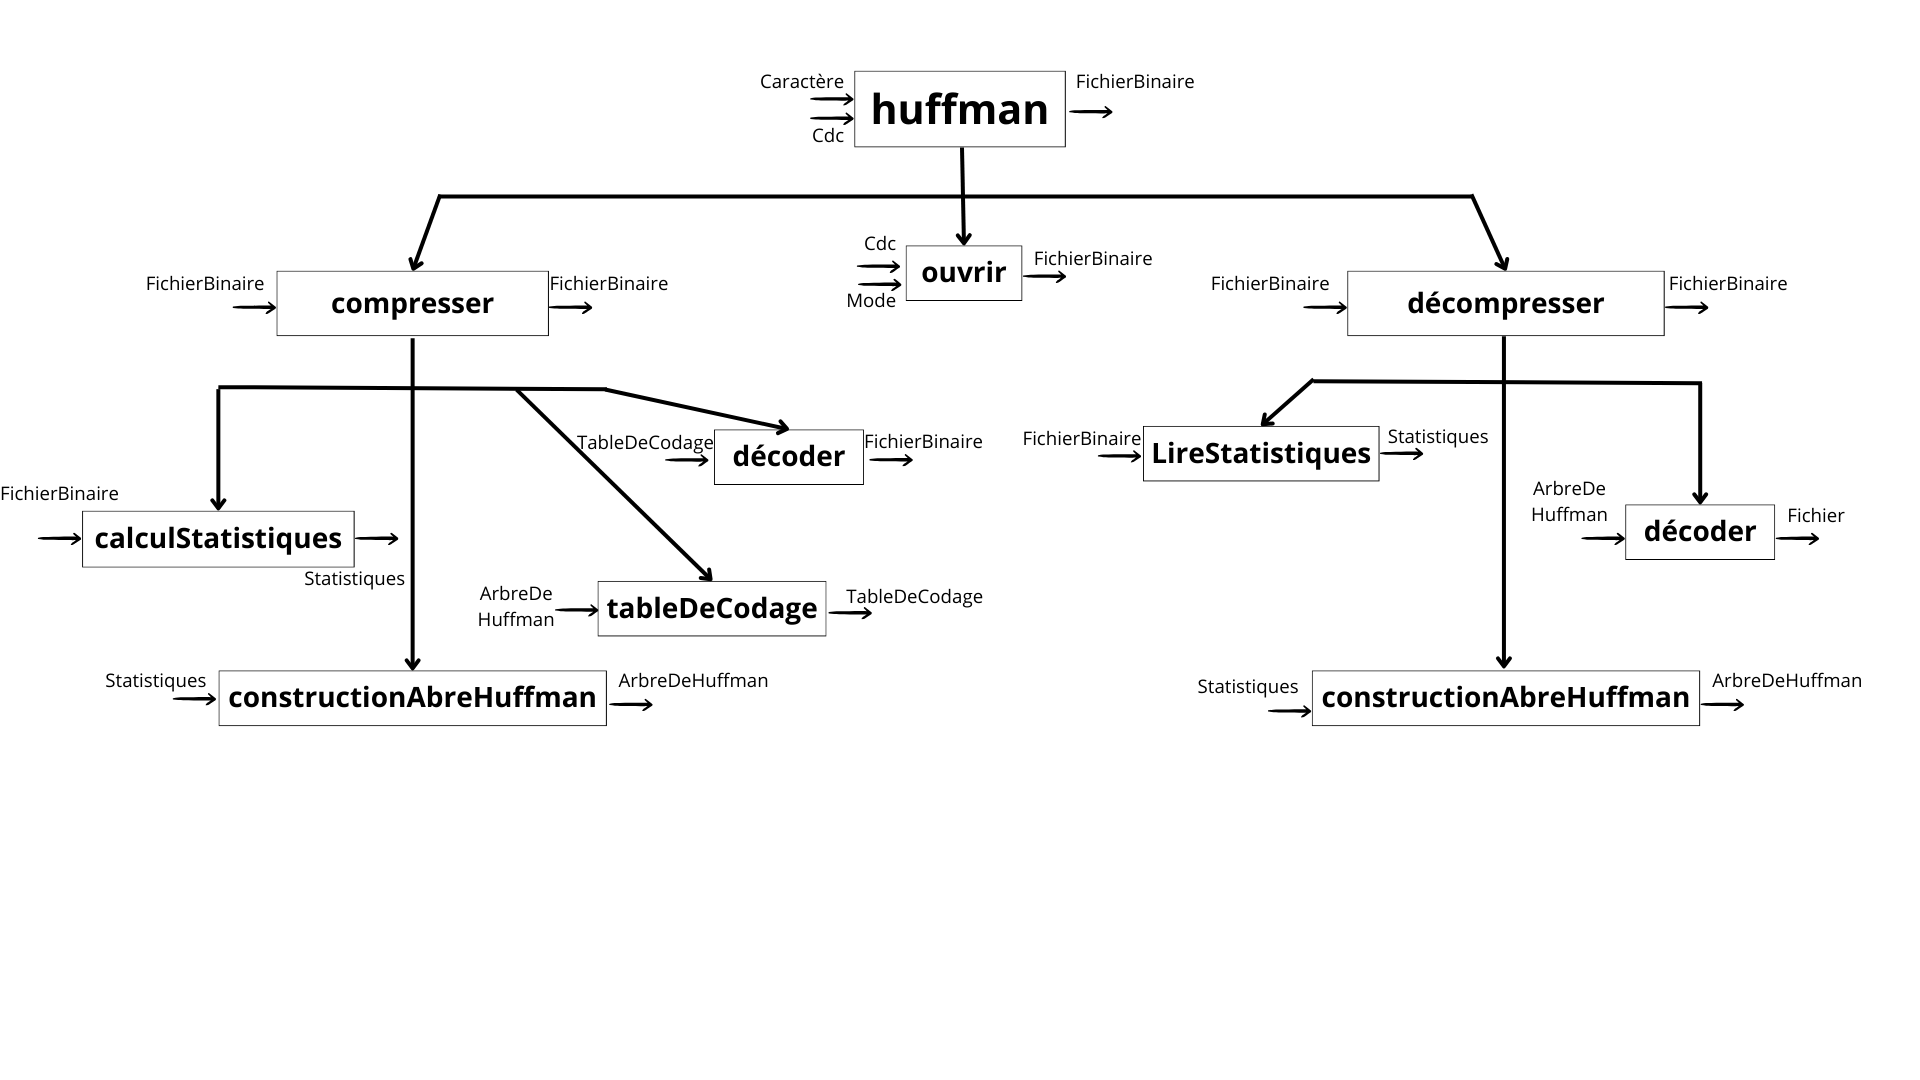
\includegraphics[width=\textwidth]{parties/analyse/Analyse descendante/huffman.png}
    \caption{Analyse descendante}
\end{figure}

\section{Conception}

\subsection{Conception Préliminaire}

\subsubsection{PriorityQueue}

\begin{algorithme} 
    \signatureFonction{priorityQueueEmpty}{}{PriorityQueue}{} 
\end{algorithme}

\begin{algorithme}
    \signatureProcedure{addTree}{\paramEntree{tree: HuffmanTree} \paramEntreeSortie{queue: PriorityQueue}}{}
\end{algorithme}

\begin{algorithme}
    \signatureFonction{removeTree}{queue: PriorityQueue}{Tree}
    {sizeQueue(f) > 0}
\end{algorithme}

\begin{algorithme}
    \signatureFonction{sizeQueue}{queue: PriorityQueue}{\naturel}{}
\end{algorithme}


\end{document}
